\documentclass[10pt,a4paper]{article}
\usepackage[utf8]{inputenc}
\usepackage[english,russian]{babel}
\usepackage{cmap}
\usepackage[OT1]{fontenc}
\usepackage{amsmath}
\usepackage{amsfonts}
\usepackage{amssymb}
\usepackage{graphicx}
\usepackage{float}
\usepackage{wrapfig}
\usepackage{caption}
\DeclareCaptionLabelSeparator{dot}{. }
\captionsetup{justification=centering,labelsep=dot}
\graphicspath{{pictures/}}
\DeclareGraphicsExtensions{.pdf,.png,.jpg,.eps}
\begin{document}



\textbf{10. Одновременная локализация и построение карт}\\

\textbf{10.1	Введение}\\

Эта и последующие главы посвящены одной из самых фундаментальных проблем робототехники, \textit{проблеме одновременной локализации и построения карты}. Эта проблема обычно сокращается как SLAM, и также известна как "Конкурентная картография и локализация", или CML. Проблемы SLAM возникает, когда у робота нет доступа ни к карте окружения, ни к положению. Вместо этого, все, что дано, это измерения $z_{1:t}$ и сигналы управления $u_{1:t}$. Термин «одновременная локализация и построение карт» описывает суть проблемы: в SLAM роботу требуется получить карту окружающей среды с одновременным выполнением локализации на этой карте. SLAM существенно сложнее всех проблем, которые были рассмотрены до текущего момента. Он более сложен, чем локализация, поскольку карта неизвестна и ее нужно оценивать прямо во время движения. Он сложнее построения карт, поскольку положение неизвестно, и его необходимо определить.\\

ПРОБЛЕМА ОНЛАЙН SLAM\\

С вероятностной точки зрения, есть две разновидности задачи SLAM, одинаково важных на практике. Первая известна как \textit{проблема онлайн SLAM} и заключается в оценке апостериорного распределения мгновенного значения положения по карте:\\

(10.1)
$$p(x_t,m|z_{1:t},u_{1:t})$$

Здесь $x_t$ - положение в момент времени $t$, $m$ карта, а $z_{1:t}$ и $u_{1:t}$ сигналы измерения и управления, соответственно. Такая задача называется \textit{онлайн SLAM}, поскольку включает оценку переменной, которая сохраняется в момент времени $t$. Многие алгоритмы онлайн SLAM работают последовательно, отбрасывая прошлые измерения и сигналы управления после обработки. Графическая модель онлайн SLAM показана на Рис. 10.1.

\begin{figure}[H]
	\center{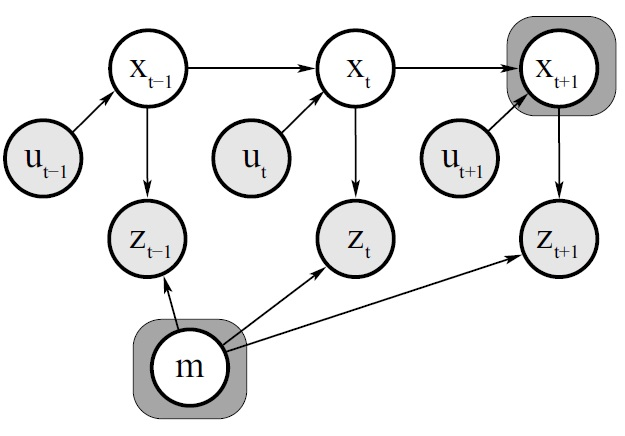
\includegraphics[width=0.7\linewidth]{101orig}}
	\caption{ ( Рис. 10.1 Графическая модель проблемы онлайн SLAM. Целью модели является оценка апостериорной вероятности по текущему положению робота, а также построение карты.))}
	\label{fig:101orig}
\end{figure}

ПОЛНАЯ ПРОБЛЕМА SLAM\\ 
Вторая проблема SLAM называется \textit{полная проблема SLAM}. В полной проблеме SLAM требуется вычислить апостериорную вероятность по всему пути $x_{1:t}$ а также карту, а не только текущее положение $x_t$ (см. также Рис. 10.2):\\

(10.2)
$$p(x_{1:t},m|z_{1:t},u_{1:t})$$

эти мелкие различия между полной и онлайн задачей SLAM влияют на алгоритмы, которые требуется сформулировать. В частности, проблема онлайн SLAM является результатом интеграции всех прошлых положений из полной проблемы SLAM:\\

(10.3)
$$p(x_t,m|z_{1:t},u_{1:t})=\int\,\int...\int p(x_{1:t},m|z_{1:t},u_{1:t})\,dx_1\,dx_2\,...dx_{t-1}$$

В онлайн SLAM эта интеграция обычно выполняется по одному положению. Это вызывает интересные изменения структуры зависимостей в SLAM, которые будут в полной мере раскрыты в следующей главе.

Второй ключевой характеристикой SLAM является способ оценки. Задачи SLAM могут содержать как непрерывный, так и дискретный вариант оценок. Непрерывная оценка относится к местоположению объектов на карте и собственным переменным положения робота. Объекты могут быть ориентирами в представлении на основе признаков или же частями объектов, обнаруженными датчиками расстояния. Дискретные способы оценок связаны с необходимостью иметь дело с соответствием объектов: при обнаружении препятствия алгоритм SLAM должен соотнести этот объект с ранее обнаруженными. Это соотношение обычно дискретно, то есть необходимо выяснить, относится ли объект к обнаруженным ранее или же нет.

\begin{figure}[H]
	\center{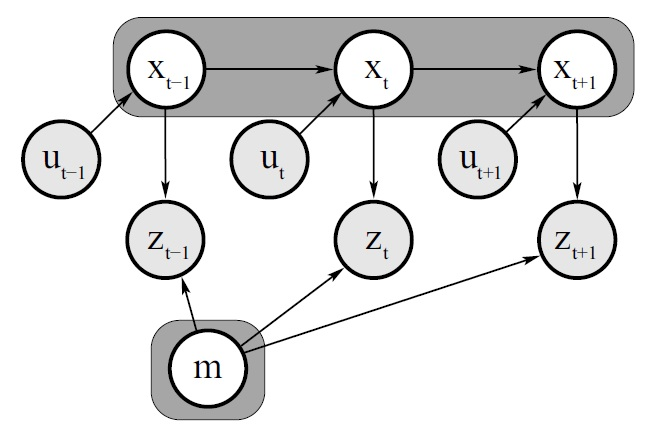
\includegraphics[width=0.7\linewidth]{102orig}}
	\caption{ ( Рис. 10.2 Графическая модель полной проблемы SLAM. Здесь вычисляется полное апостериорное распределение по всему пути робота и карте.))}
	\label{fig:102orig}
\end{figure}

Мы уже сталкивались с похожими проблемами непрерывной-дискретной оценки в предыдущих главах. Например, для локализации на основе EKF в разделе 7.4 выполняется оценку положения робота в непрерывном виде. Но, для ее осуществления необходимо установить соответствия измерений и ориентиров на карте, представленных дискретными величинами. В этой и последующей главах будут обсуждаться несколько различных методов для работы как с непрерывными, так и с дискретными частями алгоритма SLAM.

Иногда будет полезно выделять переменные соответствия в явном виде, как делалось в Главе 7 в контексте локализации. Апостериорная вероятность онлайн SLAM задана в виде\\

(10.4)
$$p(x_t,m,c_t|z_{1:t}u_{1:t})$$

а в полной задаче SLAM \\

(10.5)
$$p(x_{1:t},m,c_{1:t}|z_{1:t},u_{1:t})$$

Апостериорная вероятность в онлайн виде получается из полной апостериорной интеграцией прошлых положений робота и суммирования по всем прошлым соответствиям:\\

(10.6)
\begin{equation*}
\begin{split}
p(&x_t,m,c_t|z_{1:t},u_{1:t}) \\
&=\int\,\int...\int\sum_{c_1}\sum_{c_2}...\sum_{c_{t-1}}p(x_{1:t},m,c_{1:t}|z_{1:t},u_{1:t})\,dx_1\,dx_2...dx_{t-1}
\end{split}
\end{equation*}

В обоих версиях проблемы SLAM оценка полной апостериорной вероятности (10.4) или (10.5) является неотъемлемой частью. В полной апостериорной вероятности отображается все, что известно о карте и положении робота или пройденном пути. 

На практике, вычисление полной апостериорной вероятности обычно невыполнимо в силу следующих причин: (1) высокой размерности непрерывного пространства параметров, и (2) большого числа дискретных переменных соответствия. Многие современные алгоритмы SLAM конструируют карты с десятками тысяч признаков. Даже при известном соответствии, апостериорная вероятность только по этим картам включает вероятностные распределения с $10^5$ или более измерений. Это противоречит задаче локализации, где апостериорная вероятность оценивалась в трёхмерном непрерывном пространстве. Далее, в большинстве практических ситуаций соответствия неизвестны. Количество возможных назначений вектора всех переменных соответствия $c_{1:t}$ экспоненциально растёт за время $t$, поэтому, практические алгоритмы SLAM, способные решить проблему соответствия, должны быть основаны на приближениях.

Задача SLAM будет обсуждаться в большинстве следующих глав. В этой главе будет разработан алгоритм EKF для онлайн SLAM. Большая часть материала основана на разделе 3.3, где были описаны EKF, и раздела 7.4, где алгоритм EKF применялся в задаче локализации мобильного робота. Также будет описано развитие алгоритмов EKF, позволяющее использовать EKF для SLAM с известным соответствием, а затем - обобщить для случая с неизвестным соответствием.\\

\textbf{10.2 SLAM с обобщёнными фильтрами Калмана}\\

\textbf{10.2.1  Исходные условия и допущения}\\

Исторически самый ранний и, возможно, наиболее важный алгоритм SLAM основан на обобщённом фильтре Калмана (EKF). Напомним, в алгоритме EKF SLAM обобщенный калмановский фильтр применяется для онлайн SLAM, выполняя ассоциацию данных на основе максимального правдоподобия. В силу этого, EKF SLAM подвержен некоторым ограничениям аппроксимации и допущениям:\\

КАРТЫ НА ОСНОВЕ ПРИЗНАКОВ\\

Карты в EKF SLAM \textit{основаны на признаках} и состоят из точечных ориентиров. В силу ограничений вычислительной мощности, количество точечных ориентиров достаточно мало (обычно менее 1000). Более того, методы на основе EKF не слишком хорошо работают с  ориентирами, которые трудно различить между собой. Поэтому  требуется существенная доработка детекторов признаков EKF SLAM, иногда используя в качестве ориентиров искусственные маяки.\\

ГАУССОВСКИЙ ШУМ\\

Как любой алгоритм EKF, EKF SLAM использует допущение о наличии \textit{гауссовского шума} в движении и восприятии робота. Величина неопределённости в апостериорной вероятности должна быть относительно малой, поскольку в противном случае линеаризация EKF начинает генерировать неприемлемые ошибки.\\

ПОЛОЖИТЕЛЬНАЯ ИНФОРМАЦИЯ\\

Алгоритм EKF SLAM, так же как алгоритм локализации EKF, обсуждаемый в разделе 7.4, способен обрабатывать только \textit{положительные} наблюдения ориентиров. Он неспособен воспринимать
отрицательную информацию, возникающую из отсутствия ориентиров в измерениях датчика. Это является прямым следствием использования для отображения гауссовых оценок и обсуждалась в разделе 7.4.\\

\textbf{10.2.2 SLAM с известным соответствием}\\

Алгоритм SLAM для случая с известным соответствием решает только непрерывную часть проблемы SLAM. Его вывод во многом согласуется с выводом алгоритма локализации на основе EKF из раздела 7.4, но с одним ключевым различием: вдобавок к оценке положения робота $x_t$, алгоритм EKF SLAM также оценивает координаты всех ориентиров, которые встретились на пути. Это делает необходимым включение координат ориентира в вектор состояния.\\

КОМБИНИРОВАННЫЙ ВЕКТОР СОСТОЯНИЯ\\

Для удобства, назовём вектор состояния, включающий положение робота и карту \textit{комбинированным вектором состояния}, и обозначим как $y_t$. Комбинированный вектор задан в виде\\
(10.7)
\begin{equation*}
\begin{split}
y_t&=\left(\begin{array}{c} x_t\\
m  
\end{array} \right)\\
&=(x\,\,y\,\,\theta\,\,m_{1,x}\,\,m_{1,y}\,\,s_1\,\,m_{2,x}\,\,m_{2,y}\,\,s_2...m_{N,x}\,\,m_{N,y}\,\,s_N)^T
\end{split}
\end{equation*}

Здесь $x$, $y$ и $\theta$ означают координаты робота в момент времени $t$ (не следует путать с переменными состояния $x_t$ и $y_t$), $m_{i,x}$, $m_{i,y}$ - координаты $i$-го ориентира при $i = 1,...,N$ , а $s_i$  - сигнатура ориентира. Размерность этого вектора состояния составляет $3N+3$, где $N$ означает количество ориентиров на карте.

\begin{table}[H]
\begin{center}
\begin{tabular}{|l|}
\hline
{}\\
1: \textbf{Algorithm EKF\_SLAM\_known\_correspondences}$(\mu_{t-1},\varSigma_{t-1},u_t,z_t,c_t):$ \\
2:\hspace{5mm}
\begin{minipage}{0.2\textwidth}
\begin{equation*}
F_x=\left(\begin{array}{cccc} 1&0&0&0...0\\
0&1&0&0...0\\
0&0&1&\underbrace{0...0}_{3N}\\ 
\end{array} \right)
\end{equation*}
\end{minipage}\\
3:\hspace{5mm}
\begin{minipage}{0.2\textwidth}
\begin{equation*}
\bar{\mu}_t=\mu_{t-1}+F_x^T\left(\begin{array}{c} 
-\frac{v_t}{\omega_t}\sin \mu_{t-1,\theta}+\frac{v_t}{\omega_t}\sin(\mu_{t-1,\theta}+\omega_t\varDelta t)\\
\frac{v_t}{\omega_t}\cos\mu_{t-1,\theta}-\frac{v_t}{\omega_t}\cos(\mu_{t-1,\theta}+\omega_t\varDelta t)\\
\omega_t\varDelta t\\ 
\end{array} \right)\\
\end{equation*}
\end{minipage}\\
4:\hspace{5mm}
\begin{minipage}{0.2\textwidth}
\begin{equation*}
G_t=I+F_x^T\left(\begin{array}{ccc} 
0&0&-\frac{v_t}{\omega_t}\cos \mu_{t-1,\theta}+\frac{v_t}{\omega_t}\cos(\mu_{t-1,\theta}+\omega_t\varDelta t)\\
0&0&-\frac{v_t}{\omega_t}\sin\mu_{t-1,\theta}+\frac{v_t}{\omega_t}\sin(\mu_{t-1,\theta}+\omega_t\varDelta t)\\
0&0&0\\ 
\end{array} \right)\,F_x\\
\end{equation*}
\end{minipage}\\
5:\hspace{5mm}$\bar{\varSigma}_t=G_t\,\varSigma_{t-1}\,G_t^T+F_x^T\,R_t\,F_x$\\
6:\hspace{5mm}
\begin{minipage}{0.2\textwidth}
\begin{equation*}
Q_t=\left(\begin{array}{ccc} \sigma_r^2&0&0\\
0&\sigma_\phi^2&0\\
0&0&\sigma_s^2\\
\end{array} \right)\\
\end{equation*}
\end{minipage}\\
7:\hspace{5mm}$\textit{для всех наблюдаемых признаков}\,\,z_t^i=(r_t^i\,\,\phi_t^i\,\,s_t^i)^T\,\,\textit{do}$\\
8:\hspace{10mm}$j=c_t^i$\\
9:\hspace{10mm}$\textit{если признак j не наблюдался ранееe}$\\
10:\hspace{15mm}
\begin{minipage}{0.2\textwidth}
\begin{equation*}
\left(\begin{array}{c} \bar{\mu}_{j,x}\\
\bar{\mu}_{j,y}\\
\bar{\mu}_{j,s}\\
\end{array} \right)\\
=\left(\begin{array}{c} \bar{\mu}_{t,x}\\
\bar{\mu}_{t,y}\\
s_t^i\\
\end{array} \right)\\
+\left(\begin{array}{c} r_t^i\,\cos(\phi_t^i+\bar{\mu}_{t,\theta})\\
r_t^i\,\sin(\phi_t^i+\bar{\mu}_{t,\theta})\\
0\\
\end{array} \right)
\end{equation*}
\end{minipage}\\
11:\hspace{9mm}$\textit{endif}$\\
12:\hspace{9mm}
\begin{minipage}{0.2\textwidth}
\begin{equation*}
\delta=\left(\begin{array}{c} \delta_x\\
\delta_y\\
\end{array} \right)\\
=\left(\begin{array}{c} \bar{\mu}_{j,x}-\bar{\mu}_{t,x}\\
\bar{\mu}_{j,y}-\bar{\mu}_{t,y}\\
\end{array} \right)\\
\end{equation*}
\end{minipage}\\
13:\hspace{9mm}$q=\delta^T\,\delta$\\
14:\hspace{9mm}
\begin{minipage}{0.2\textwidth}
\begin{equation*}
\hat{z}_t^i=\left(\begin{array}{c} \sqrt{q}\\
\text{atan2}(\delta_y,\delta_x)-\bar{\mu}_{t,\theta}\\
\bar{\mu}_{j,s}
\end{array} \right)\\
\end{equation*}
\end{minipage}\\
15:\hspace{9mm}
\begin{minipage}{0.2\textwidth}
\begin{equation*}
F_{x,j}=\left(\begin{array}{cccccccc} 
1&0&0&0...0&0&0&0&0...0\\
0&1&0&0...0&0&0&0&0...0\\
0&0&1&0...0&0&0&0&0...0\\
0&0&0&0...0&1&0&0&0...0\\
0&0&0&0...0&0&1&0&0...0\\
0&0&0&\underbrace{0...0}_{3j-3}&0&0&1&\underbrace{0...0}_{3N-3j}
\end{array} \right)\\
\end{equation*}
\end{minipage}\\
16:\hspace{9mm}
\begin{minipage}{0.2\textwidth}
\begin{equation*}
H_t^i=\frac{1}{q}\,\left(\begin{array}{cccccc} -\sqrt{q}\delta_x&-\sqrt{q}\delta_y&0&+\sqrt{q}\delta_x&\sqrt{q}\delta_y&0\\
\delta_y&-\delta_x&-q&-\delta_y&+\delta_x&0\\
0&0&0&0&0&q
\end{array} \right)\\\,F_{x,j}
\end{equation*}
\end{minipage}\\
17:\hspace{9mm}$K_t^i=\bar{\varSigma}_t H_t^{iT}(H_t^i\bar{\varSigma}_t H_t^{iT}+Q_t)^{-1}$\\
18:\hspace{9mm}$\bar{\mu}_t=\bar{\mu}_t+K_t^i(z_t^i-\hat{z}_t^i)$\\
19:\hspace{9mm}$\bar{\varSigma}_t=(I-K_t^iH_t^i)\bar{\varSigma}_t$\\
20:\hspace{4mm}$\textit{endfor}$\\
21:\hspace{4mm}$\mu_t=\bar{\mu}_t$\\
22:\hspace{4mm}$\varSigma_t=\bar{\varSigma}_t$\\
23:\hspace{4mm}$\textit{return}\,\,\mu_t,\varSigma_t$\\
{}\\
\hline
\end{tabular}
\caption{(Таблица 10.1 Алгоритм EKF для задачи SLAM с известными соответствиями.)}
\end{center}
\end{table}

Очевидно, для любого разумного числа $N$ этот вектор существенно больше вектора положений, оценённого в разделе 7.4, где впервые был описан алгоритм локализации EKF. EKF SLAM вычисляет онлайновую апостериорную вероятность $p(y_t|z_{1:t}, u_{1:t})$.

Алгоритм EKF SLAM приводится в Таблице 10.1, и явно похож на алгоритм локализации EKF в Таблице 7.2. В строках со 2 до 5 используется обновление движения, а в строках с 6 до 20 учитывается вектор измерения. 

В строках с 3 по 5 показатели математического ожидания и ковариации применяются к модели движения. Эта операция затрагивает только элементы распределения прогноза, связанные с положением робота. Она оставляет неизменными все переменные математического ожидания и ковариации для карты, а также ковариации между положением и картой.  В строках с 7 по 20 выполняется проход по всем измерениям.  Проверка в строке 9 возвращает истину только для ориентиров, у которых отсутствует первичная оценка местоположения. Для таких ориентиров в строке 10 выполняется инициализация местоположения проекцией, полученной из соответствующих измерений расстояния и направления. Как мы обсудим ниже, этот шаг важен для линеаризации в EKF, но не нужен в линейных фильтрах Калмана. Для каждого измерения «ожидаемое» измерение вычисляется в строке 14, а соответствующее усиление Калмана вычисляются в строке 17. Заметим, что усиление Калмана является матрицей размера 3 на $3N + 3$. Эта матрица обычна не разрешена и информация распространяется через всю оценку состояния. Затем обновление фильтра происходит в строках с 18 по 19, где степень новизны сворачивается обратно в значение оценки робота.

Тот факт, что усиление Калмана в полной мере распространяется на все переменные состояния, а не только на наблюдаемый ориентир и положение робота, очень важен. В SLAM наблюдение ориентира не просто улучшает оценку позиции этого ориентира, но и других ориентиров из-за изменения оценки положения робота. Наблюдение ориентира улучшает оценку положения робота, и устраняет некоторую неопределённость местоположения прежде наблюдаемых ориентиров. Положительной стороной здесь является отсутствие явной необходимости моделировать прошлые положения, которая бы привела в область полной задачи SLAM и сделала EKF оффлайновым алгоритмом. Вместо этого, зависимость отражается гауссовым апостериорным распределением, а именно, элементами вне главной диагонали матрицы ковариации $\varSigma_t$.

На Рис. 10.3 показан алгоритм EKF SLAM для вымышленного примера. Робот выполняет навигацию из стартового положения в начале координат. По мере движения неопределённость возрастает, что показано эллипсами неопределённостями возрастающего диаметра. Робот также воспринимает близлежащие ориентиры и определяет для них значение неопределённость, которая сочетает постоянную неопределённостью измерения и увеличивающуюся неопределённость положения. В результате, значение неопределённости определения местоположения ориентира со временем растёт.  Фактически, это происходит параллельно изменению значения неопределённости положения в момент наблюдения ориентира. Интересный момент показан на Рис. 10.3d. Здесь робот наблюдает ориентир, который уже наблюдался в самом начале картографирования и местоположение которого относительно хорошо известно. 

\begin{figure}[H]
	\center{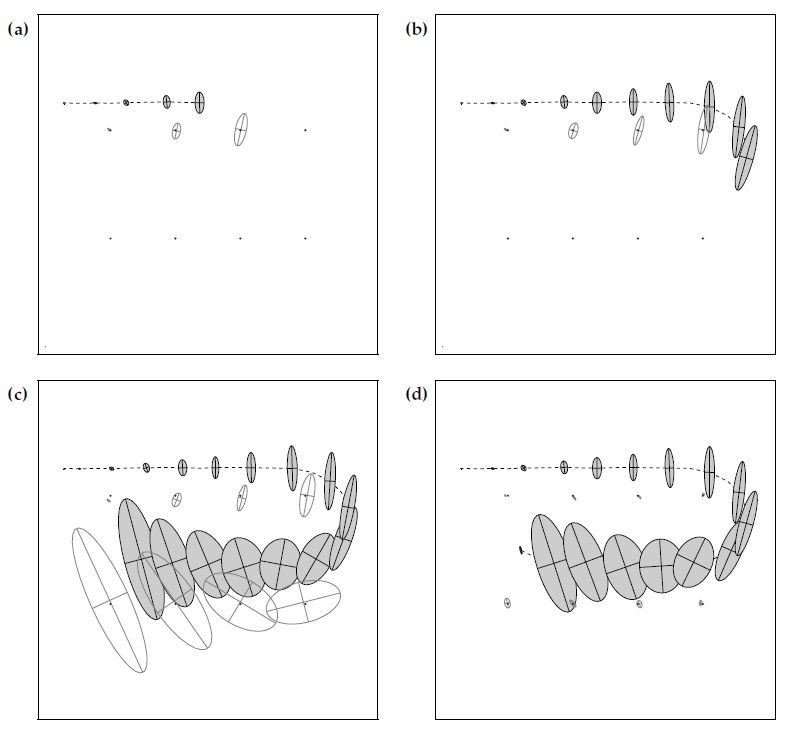
\includegraphics[width=0.86\linewidth]{103orig}}
	\caption{ ( Рис. 10.3 EKF в приложении проблемы онлайн SLAM. Путь робота обозначен пунктирной точечной линией, оценка позиций показана заштрихованными эллипсами. Восемь различимых между собой ориентиров с неизвестным местоположением показаны маленькими точками, а их оценки местоположения - белыми эллипсами. На схемах (a)–(c) неопределённость позиции робота возрастает, как и неопределённость положения ориентиров, с которыми он сталкивается. На схеме (d) робот снова обнаруживает первый ориентир, и неопределённость всех ориентиров уменьшается, как и неопределённость текущего положения. Изображение принадлежит Майклу Монтемерло из Стенфордского университета (Michael Montemerlo, Stanford University).))}
	\label{fig:103orig}
\end{figure}

С помощью этого наблюдения ошибка положения робота уменьшается, как показано на Рис. 10.3d. Обратите внимание на очень малый размер эллипса неопределённости для финального положения робота! Это наблюдение также уменьшает степень неопределённости для остальных ориентиров на карте. Так происходит из-за наличия корреляции в ковариационной матрице гауссовского апостериорного распределения. Поскольку большая часть неопределённости в ранее наблюдаемых ориентирах вызывается положением робота, и, поскольку её значение сохраняется со временем, оценки местоположения этих ориентиров коррелируют. При сборе информации о положении робота корреляция распространяется на все уже обнаруженные ориентиры. Этот эффект является, возможно, самой важной характеристикой апостериорной вероятности SLAM. Информация, помогающая локализовать робота, распространяется по карте и, в результате, улучшает локализацию ориентиров на карте.\\

\textbf{10.2.3 Математический вывод EKF SLAM}\\

Вывод алгоритма EKF SLAM для случая с известным соответствием в значительной степени походит на вывод алгоритма локализации EKF в разделе 7.4. Ключевая разница состоит в дополненном векторе состояния, который сейчас включает все ориентиры вдобавок к положению робота.

В SLAM начальное положение считается началом системы координат. Это определение произвольно, поэтому может быть заменено некоторыми координатами. Местоположение ориентиров изначально неизвестно. Оценка гипотезы выражена следующими начальными математическим ожиданием и ковариацией:\\

(10.8)
\begin{minipage}{0.2\textwidth}
\begin{equation*}
\mu_0=\left(\begin{array}{ccccc}0&0&0&\ldots&0 
\end{array} \right)^T\\
\end{equation*}
\end{minipage}

(10.9)
\begin{minipage}{0.2\textwidth}
\begin{equation*}
F_{x,j}=\left(\begin{array}{cccccc} 
0&0&0&0&\ldots&0\\
0&0&0&0&\ldots&0\\
0&0&0&0&\ldots&0\\
0&0&0&\infty&\ldots&0\\
\vdots&\vdots&\vdots&\vdots&\ddots&\vdots\\
0&0&0&0&\ldots&\infty\\
\end{array} \right)\\
\end{equation*}
\end{minipage}

Ковариационная матрица имеет размер $(3N + 3)\times(3N + 3)$. Она состоит из маленькой нулевой матрицы $3\times3$ для переменных положения робота. Все остальные значения ковариации бесконечны.

При движении робота вектор состояния меняется согласно стандартной идеальной модели на основе скоростей (см. выражения (5.13) и (7.4)). В SLAM эта модель движения расширяется до дополненного вектора состояния:\\

(10.10)
\begin{minipage}{0.2\textwidth}
\begin{equation*}
y_t=y_{t-1}+\left(\begin{array}{c} 
-\frac{v_t}{\omega_t}\sin\theta+\frac{v_t}{\omega_t}\sin(\theta+\omega_t\varDelta t)\\	\frac{v_t}{\omega_t}\cos\theta-\frac{v_t}{\omega_t}\cos(\theta+\omega_t\varDelta t)\\	\omega_t\varDelta t+\gamma_t\varDelta t\\
0\\
\vdots\\
0\\
\end{array} \right)\\
\end{equation*}
\end{minipage}

Переменные $x$, $y$ и $\theta$ определяют положение робота в $y_{t-1}$. Поскольку движение влияет только на положение робота и все ориентиры остаются на месте, только первые три элемента обновления не равны нулю. Это позволяет записать равенство более компактно:\\

(10.11)
\begin{minipage}{0.2\textwidth}
\begin{equation*}
y_t=y_{t-1}+F_x^T\,\left(\begin{array}{c} 
-\frac{v_t}{\omega_t}\sin\theta+\frac{v_t}{\omega_t}\sin(\theta+\omega_t\varDelta t)\\	\frac{v_t}{\omega_t}\cos\theta-\frac{v_t}{\omega_t}\cos(\theta+\omega_t\varDelta t)\\	\omega_t\varDelta t+\gamma_t\varDelta t\\
\end{array} \right)\\
\end{equation*}
\end{minipage}

Здесь $F_x$ - матрица, проецирующая трёхмерный вектор состояния в вектор размерности $3N + 3$.\\

(10.12)
\begin{minipage}{0.2\textwidth}
\begin{equation*}
F_x=\left(\begin{array}{cccc} 
1&0&0&0\,\,...\,\,0\\
0&1&0&0\,\,...\,\,0\\
0&0&1&\underbrace{0\,\,...\,\,0}_{3N\,\,\text{columns}}\\
\end{array} \right)\\
\end{equation*}
\end{minipage}

Полная модель движения с учётом шумов выглядит следующим образом\\

(10.13)
\begin{minipage}{0.2\textwidth}
\begin{equation*}
y_t=\underbrace {y_{t-1}+F_x^T\,\left(\begin{array}{c} 
-\frac{v_t}{\omega_t}\sin\theta+\frac{v_t}{\omega_t}\sin(\theta+\omega_t\varDelta t)\\	\frac{v_t}{\omega_t}\cos\theta-\frac{v_t}{\omega_t}\cos(\theta+\omega_t\varDelta t)\\	\omega\varDelta t\\
\end{array} \right)\\}_{g(u_t,y_{t-1})}+\mathcal{N}(0,F_x^T\,R_t\,F_x)
\end{equation*}
\end{minipage}

где $F_x^T\,R_t\,F_x$ расширяет ковариационную матрицу до размерности полного вектора состояния в квадрате.

Как обычно в EKFs, функция движения $g$ аппроксимируется, используя первую степень разложения в ряд Тейлора\\

(10.14)
$$g(u_t,y_{t-1})\approx g(u_t,\mu_{t-1})+G_t(y_{t-1}-\mu_{t-1})$$

где якобиан $G_t=g'(u_t,\mu_{t-1})$ является производной $g$ по отношению к
$y_{t-1}$ по $u_t$ и $\mu_{t-1}$, как в Выражении (7.7).

Очевидно, аддитивная форма выражения (10.13) позволяет разложить этот якобиан в матрицу тождественного преобразования $(3N+3)\times(3N+3)$ (производная $y_{t-1}$) плюс якобиан низкой размерности $g_t$, характеризующий изменение положения робота:\\

(10.15)
$$G_t=I+F_x^T\,g_t\,F_x$$

с\\

(10.16)
\begin{minipage}{0.2\textwidth}
\begin{equation*}
g_t=\left(\begin{array}{ccc} 
0&0&-\frac{v_t}{\omega_t}\cos\mu_{t-1,\theta}+\frac{v_t}{\omega_t}\cos(\mu_{t-1,\theta}+\omega_t\varDelta t)\\	0&0&-\frac{v_t}{\omega_t}\sin\mu_{t-1,\theta}+\frac{v_t}{\omega_t}\sin(\mu_{t-1,\theta}+\omega_t\varDelta t)\\	0&0&0\\
\end{array} \right)\\
\end{equation*}
\end{minipage}

Вставка этих приближений в стандартный алгоритм EKF показана в строках с 2 по 5 Таблицы 10.1. Очевидно, некоторые матрицы, перемножаемые в строке 5, разреженные, и это следует использовать при реализации алгоритма.  Результат обновления даёт математическое ожидание $\bar{\mu}_t$ и ковариацию оценки $\bar{\varSigma}_t$  в момент времени $t$ после обновления фильтра управляющим сигналом $u_t$, но до учёта измерения $z_t$.

Вывод обновления измерения похож на аналогичный из раздела 7.4. В частности, дана следующая модель измерения\\

(10.17)
\begin{minipage}{0.2\textwidth}
\begin{equation*}
z_t^i=\underbrace {\left(\begin{array}{c} 
\sqrt{(m_{j,x}-x)^2+(m_{j,y}-y)^2}\\
\text{atan2}(m_{j,y}-y,m_{j,x}-x)-\theta\\	m_{j,s}\\
\end{array} \right)\\}_{h(y_t,j)}+\mathcal{N}(0,\underbrace{\left(\begin{array}{ccc} \sigma_r&0&0\\
0&\sigma_\phi&0\\
0&0&\sigma_s\\
\end{array} \right)}_{Q_t})
\end{equation*}
\end{minipage}

Здесь $x$, $y$ и $\theta$ определяют положение робота, $i$ –индекс отдельного наблюдения ориентира в измерении $z_t$, а $j=c_t^i$ индекс наблюдаемого ориентира в момент времени $t$. Переменная $r$ обозначает расстояние до ориентира, $\phi$ -  угол направления на ориентир, а $s$ – сигнатура ориентира. Элементы $\sigma_r$, $\sigma_\phi$, и $\sigma_s$ – это ковариации соответствующих шумов измерений.

Это выражение аппроксимируется линейной функцией\\

(10.18)
$$h(y_t,j)\approx h(\bar{\mu}_t,j)+H_t^i(y_t-\bar{\mu}_t)$$

Здесь $H_t^i$ - производная $h$ по полному вектору состояний $y_t$. Поскольку $h$ зависит от двух элементов этого вектора состояния – положения робота $x_t$ и местоположения $j$-го ориентира $m_j$, переменная умножается на якобиан с низкой размерностью $h_t^i$ и матрицу $F_{x,j}$, которая проектирует $h_t^i$ в матрицу размерности полного вектора состояния:\\

(10.19)
$$H_t^i=h_t^i\,\,F_{x,j}$$

Здесь $h_t^i$ – якобиан функции $h(y_t,j)$ по $\bar{\mu}_t$, вычисленный по переменным состояния $x_t$ и $m_j$:

(10.20)
\begin{minipage}{0.2\textwidth}
\begin{equation*}
h_t^i=\left(\begin{array}{cccccc} 
\frac{\bar{\mu}_{t,x}-\bar{\mu}_{j,x}}{\sqrt{q_t}}&\frac{\bar{\mu}_{t,y}-\bar{\mu}_{j,y}}{\sqrt{q_t}}&0&\frac{\bar{\mu}_{j,x}-\bar{\mu}_{t,x}}{\sqrt{q_t}}&\frac{\bar{\mu}_{j,y}-\bar{\mu}_{t,y}}{\sqrt{q_t}}&0\\	\frac{\bar{\mu}_{j,y}-\bar{\mu}_{t,y}}{q_t}&\frac{\bar{\mu}_{t,x}-\bar{\mu}_{j,x}}{q_t}&-1&\frac{\bar{\mu}_{t,y}-\bar{\mu}_{j,y}}{q_t}&\frac{\bar{\mu}_{j,x}-\bar{\mu}_{t,x}}{q_t}&0\\
0&0&0&0&0&1\\
\end{array} \right)\\
\end{equation*}
\end{minipage}\\

Скаляр $q_t=(\bar{\mu}_{j,x}-\bar{\mu}_{t,x})^2+(\bar{\mu}_{j,y}-\bar{\mu}_{t,y})^2$, и $j=c_t^i$ составляют ориентир, соответствующий измерению $z_t^i$. Матрица $F_{x,j}$ имеет размерность $6\times(3N+3)$ и отображает матрицу с малым количеством измерений  $h_t^i$  в матрицу размерности $3\times(3N+3)$:\\

(10.21)
\begin{minipage}{0.2\textwidth}
\begin{equation*}
F_{x,j}=\left(\begin{array}{cccccccc} 
1&0&0&0...0&0&0&0&0...0\\
0&1&0&0...0&0&0&0&0...0\\
0&0&1&0...0&0&0&0&0...0\\
0&0&0&0...0&1&0&0&0...0\\
0&0&0&0...0&0&1&0&0...0\\
0&0&0&\underbrace{0...0}_{3j-3}&0&0&1&\underbrace{0...0}_{3N-3j}
\end{array} \right)\\
\end{equation*}
\end{minipage}

Эти выражения составляют основу вычисления усиления Калмана в строках с 8 по 17 алгоритма EKF SLAM в Таблице 10.1, с одним важным дополнением. Когда ориентир обнаруживается в первый раз, его начальная оценка положения в Выражении (10.8) ухудшает линеаризации. Это происходит потому, что при инициализации по умолчанию в (10.8), точка линеаризации функции $h$ представлена как 
$(\hat{\mu}_{j,x}\,\,\hat{\mu}_{j,y}\,\,\hat{\mu}_{j,s})^T=(0\,\,0\,\,0)^T$, что является очень плохой функцией оценки местоположения ориентира. 
Лучшая функция оценки ориентира дана в строке 10 Таблицы 10.1.
Здесь инициализация оценки ориентира происходит в виде  $(\hat{\mu}_{j,x}\,\,\hat{\mu}_{j,y}\,\,\hat{\mu}_{j,s})^T$ с помощью прогнозируемого положения. Эта величина выводится из прогнозируемого положения робота и переменных измерения для ориентира\\

(10.22)
\begin{minipage}{0.2\textwidth}
\begin{equation*}
\left(\begin{array}{c} \bar{\mu}_{j,x}\\
\bar{\mu}_{j,y}\\
\bar{\mu}_{j,s}\\
\end{array} \right)\\
=\left(\begin{array}{c} \bar{\mu}_{t,x}\\
\bar{\mu}_{t,y}\\
s_t^i\\
\end{array} \right)\\
+\left(\begin{array}{c} r_t^i\,\cos(\phi_t^i+\bar{\mu}_{t,\theta})\\
r_t^i\,\sin(\phi_t^i+\bar{\mu}_{t,\theta})\\
0\\
\end{array} \right)
\end{equation*}
\end{minipage}\\
 \\
Заметим, что такая инициализация возможна только потому, что функция измерения $h$ взаимно однозначна. Измерения представлены двухмерными величинами, так же, как местоположения ориентиров. В случае, когда измерение имеет меньшую размерность, чем координаты ориентира, $h$ является проекцией и вычислить осмысленное значение ожидания для $(\bar{\mu}_{j,x}\,\,\bar{\mu}_{j,y}\,\,\bar{\mu}_{j,s})^T$ на основе единственного измерения невозможно. Так происходит, например, в реализации SLAM в компьютерном зрении, поскольку при использовании камер для ориентира часто вычисляется только угол направления, но не расстояние. Напротив, в SLAM обычно выполняется интеграция нескольких наблюдений с последующей триангуляцией для определения подходящей начальной оценки местоположения. В литературе по SLAM такая проблема называется  SLAM \textit{только по направлению} и позже будет обсуждаться в одном из упражнений (страница 334???).

Наконец, заметим, что алгоритм EKF требует объёма памяти, квадратично зависящего от $N$, количества ориентиров на карте. Время обновления также квадратично к $N$. Квадратичная сложность обновления возникает из-за перемножения матриц, которое имеет место в различных тактах алгоритма EKF.

\begin{table}[H]
\begin{center}
\begin{tabular}{|l|}
\hline
{}\\
1: \textbf{Algorithm EKF\_SLAM\_known\_correspondences}$(\mu_{t-1},\varSigma_{t-1},u_t,z_t,c_t):$ \\
2:\hspace{5mm}$N_t=N_{t-1}$\\
3:\hspace{5mm}
\begin{minipage}{0.2\textwidth}
				\begin{equation*}
				F_x=\left(\begin{array}{cccc} 1&0&0&0...0\\
				0&1&0&0...0\\
				0&0&1&0...0\\ 
				\end{array} \right)
				\end{equation*}
\end{minipage}\\
4:\hspace{5mm}
\begin{minipage}{0.2\textwidth}
				\begin{equation*}
				\bar{\mu}_t=\mu_{t-1}+F_x^T\left(\begin{array}{c} 
				-\frac{v_t}{\omega_t}\sin \mu_{t-1,\theta}+\frac{v_t}{\omega_t}\sin(\mu_{t-1,\theta}+\omega_t\varDelta t)\\
				\frac{v_t}{\omega_t}\cos\mu_{t-1,\theta}-\frac{v_t}{\omega_t}\cos(\mu_{t-1,\theta}+\omega_t\varDelta t)\\
				\omega_t\varDelta t\\ 
				\end{array} \right)\\
				\end{equation*}
\end{minipage}\\
5:\hspace{5mm}
\begin{minipage}{0.2\textwidth}
				\begin{equation*}
				G_t=I+F_x^T\left(\begin{array}{ccc} 
				0&0&-\frac{v_t}{\omega_t}\cos \mu_{t-1,\theta}+\frac{v_t}{\omega_t}\cos(\mu_{t-1,\theta}+\omega_t\varDelta t)\\
				0&0&-\frac{v_t}{\omega_t}\sin\mu_{t-1,\theta}+\frac{v_t}{\omega_t}\sin(\mu_{t-1,\theta}+\omega_t\varDelta t)\\
				0&0&0\\ 
				\end{array} \right)\,F_x\\
				\end{equation*}
\end{minipage}\\
6:\hspace{5mm}$\bar{\varSigma}_t=G_t\,\varSigma_{t-1}\,G_t^T+F_x^T\,R_t\,F_x$\\
7:\hspace{5mm}
\begin{minipage}{0.2\textwidth}
				\begin{equation*}
				Q_t=\left(\begin{array}{ccc} \sigma_r^2&0&0\\
				0&\sigma_\phi^2&0\\
				0&0&\sigma_s^2\\
				\end{array} \right)\\
				\end{equation*}
\end{minipage}\\
8:\hspace{5mm}$\textit{for all observed features}\,\,z_t^i=(r_t^i\,\,\phi_t^i\,\,s_t^i)^T\,\,\textit{do}$\\
9:\hspace{10mm}
\begin{minipage}{0.2\textwidth}
				\begin{equation*}
				\left(\begin{array}{c} \bar{\mu}_{N_t+1,x}\\
				\bar{\mu}_{N_t+1,y}\\
				\bar{\mu}_{N_t+1,s}\\
				\end{array} \right)\\
				=\left(\begin{array}{c} \bar{\mu}_{t,x}\\
				\bar{\mu}_{t,y}\\
				s_t^i\\
				\end{array} \right)\\
				+r_t^i\left(\begin{array}{c} \cos(\phi_t^i+\bar{\mu}_{t,\theta})\\
				\sin(\phi_t^i+\bar{\mu}_{t,\theta})\\
				0\\
				\end{array} \right)
				\end{equation*}
\end{minipage}\\
10:\hspace{9mm}$\textit{for}\,\,k=1\,\,\textit{to}\,\,N_t+1\,\,\textit{do}$\\
11:\hspace{9mm}
\begin{minipage}{0.2\textwidth}
				\begin{equation*}
				\delta_k=\left(\begin{array}{c} \delta_{k,x}\\
				\delta_{k,y}\\
				\end{array} \right)\\
				=\left(\begin{array}{c} \bar{\mu}_{k,x}-\bar{\mu}_{t,x}\\
				\bar{\mu}_{k,y}-\bar{\mu}_{t,y}\\
				\end{array} \right)\\
				\end{equation*}
\end{minipage}\\
12:\hspace{9mm}$q_k=\delta_k^T\,\delta_k$\\
{}\\
{}\\
{}\\
\hspace{65mm}$\boxed{\textit{продолжение на следующей странице}}$\\
\hline
\end{tabular}
\end{center}
\end{table}


\begin{table}[H]
\begin{center}
\begin{tabular}{|l|}
\hline
\hspace{70mm}$\boxed{\textit{начало на предыдущей странице}}$\\
{}\\
13:\hspace{9mm}
\begin{minipage}{0.2\textwidth}
				\begin{equation*}
				\hat{z}_t^k=\left(\begin{array}{c} \sqrt{q_k}\\
				\text{atan2}(\delta_{k,y},\delta_{k,x})-\bar{\mu}_{t,\theta}\\
				\bar{\mu}_{k,s}
				\end{array} \right)\\
				\end{equation*}
\end{minipage}\\
14:\hspace{9mm}
\begin{minipage}{0.2\textwidth}
				\begin{equation*}
				F_{x,k}=\left(\begin{array}{cccccccc} 
				1&0&0&0...0&0&0&0&0...0\\
				0&1&0&0...0&0&0&0&0...0\\
				0&0&1&0...0&0&0&0&0...0\\
				0&0&0&0...0&1&0&0&0...0\\
				0&0&0&0...0&0&1&0&0...0\\
				0&0&0&0...0&0&0&1&0...0
				\end{array} \right)\\
				\end{equation*}
\end{minipage}\\
15:\hspace{9mm}
\begin{minipage}{0.2\textwidth}
				\begin{equation*}
				H_t^k=\frac{1}{q_k}\,\left(\begin{array}{cccccc} -\sqrt{q_k}\delta_{k,x}&-\sqrt{q_k}\delta_{k,y}&0&\sqrt{q_k}\delta_{k,x}&\sqrt{q_k}\delta_{k,y}&0\\
				\delta_{k,y}&-\delta_{k,x}&-1&-\delta_{k,y}&\delta_{k,x}&0\\
				0&0&0&0&0&1
				\end{array} \right)\\\,F_{x,k}
				\end{equation*}
\end{minipage}\\
16:\hspace{9mm}$\varPsi_k=H_t^k\,\bar{\varSigma}_t[H_t^k]^T+Q_t$\\
17:\hspace{9mm}$\pi_k=(z_t^i-\hat{z}_t^k)^T\,\varPsi_k^{-1}(z_t^i-\hat{z}_t^k)$\\
18:\hspace{4mm}$\textit{endfor}$\\
19:\hspace{4mm}$\pi_{N_t+1}=\alpha$\\
20:\hspace{4mm}$j(i)=\underset{k}{\text{argmin}}\,\pi_k$\\
21:\hspace{4mm}$N_t=\max\left\lbrace  N_t,j(i)\right\rbrace $\\
22:\hspace{4mm}$K_t^i=\bar{\varSigma}_t [H_t^{j(i)}]^T\varPsi_{j(i)}^{-1}$\\
23:\hspace{4mm}$\bar{\mu}_t=\bar{\mu}_t+K_t^i(z_t^i-\hat{z}_t^{j(i)})$\\
24:\hspace{4mm}$\bar{\varSigma}_t=(I-K_t^iH_t^{j(i)})\bar{\varSigma}_t$\\
25:\hspace{1mm}$\textit{endfor}$\\
26:\hspace{1mm}$\mu_t=\bar{\mu}_t$\\
27:\hspace{1mm}$\varSigma_t=\bar{\varSigma}_t$\\
28:\hspace{1mm}$\textit{return}\,\,\mu_t,\varSigma_t$\\
{}\\
\hline
\end{tabular}
\caption{(Таблица 10.2 Алгоритм EKF SLAM с соответствиями по максимальному правдоподобию и отбрасыванием выбросов.)}
\end{center}
\end{table}

\textbf{10.3	EKF SLAM с неизвестными соответствиями}\\

\textbf{10.3.1	Общий алгоритм EKF SLAM }\\

СООТВЕТСТВИЕ МЕТОДОМ МАКСИМАЛЬНОГО ПРАВДОПОДОБИЯ\\
Расширим алгоритм EKF SLAM с известными соответствиями до общего алгоритма, использующего инкрементную функцию оценки максимального правдоподобия \textit{(maximum likelihood - ML)} для определения соответствия.  В Таблице 10.2 приводится алгоритм для неизвестного соответствия.

Поскольку соответствие неизвестно, на входе алгоритма \textbf{EKF\_SLAM} отсутствует переменная соответствия $c_t$. Вместо неё включается текущий размер карты $N_{t-1}$. Обновление движения в строках с 3 по 6 эквивалентно используемому в \textbf{EKF\_SLAM\_known\_correspondences} в Таблице 10.1, но цикл обновления измерения работает по-другому. Начиная со строки 8, сначала вычисляется гипотеза для нового ориентира с индексом $N_t + 1$, на единицу больше, чем количество ориентиров на карте в данный момент времени. Местоположение нового ориентира инициализируется в строке 9 вычислением ожидаемого местоположения на основании местоположения робота, расстояния и направления в измерении. В строке 9 новому ориентиру назначается метка уже известного. Далее в строках с 10 по 18 вычисляются различные параметры обновления для всех $N_t + 1$ возможных ориентиров, включая «новые». В строке 19 устанавливается порог для создания нового ориентира. Новый ориентир создаётся, если расстояние Махаланобиса до всех существующих ориентиров на карте превышает значение $\alpha$. Затем в строке 20 выделяется соответствие максимума правдоподобия. Ели измерение связано с прежде ненаблюдаемым ориентиром, счётчик ориентиров увеличивается на единицу в строке 21, и соответствующим образом увеличиваются матрицы и векторы. Этот несколько громоздкий шаг в явном виде в Таблице 10.2 не приводится. Наконец, в строках 23 и 24 выполняется такт обновления EKF. Алгоритм \textbf{EKF\_SLAM} возвращает новое количество ориентиров $N_t$ а также математическое ожидание $\mu_t$ и ковариацию $\varSigma_t$.

Вывод алгоритма EKF SLAM напрямую следует из предыдущих преобразований. В частности, инициализация в строке 9 идентична таковой в строке 10 в алгоритме \textbf{EKF\_SLAM\_known\_correspondences} Таблицы 10.1. Строки с 10 по 18 соответствуют строкам с 12 по 17 в алгоритме \textbf{EKF\_SLAM\_known\_correspondences} с добавочными переменными $\pi_k$, необходимыми для вычисления соответствия ML. Выбор соответствия по максимуму правдоподобия в строке 20 и определение расстояния Махаланобиса в строке 17, аналогичны процедуре соответствия максимального правдоподобия, описанной в разделе 7.5. В частности, в алгоритме \textbf{EKF\_localization} в Таблице 7.3 на странице 217 ??? было использовано аналогичное выражение для определения наиболее вероятного ориентира (строка 16). Обновление измерения в строках 23 и 24 Таблицы 10.2 также повторяет алгоритм EKF с известным соответствием, при этом подразумевается, что задействованные векторы и матрицы уже имеют необходимый размер для случая, когда карта была дополнена.

Наш пример реализации \textbf{EKF\_SLAM} можно улучшить ограничением учитываемых ориентиров в строках с 10 по 18 только близко расположенными относительно робота. Более того, многие из значений и матриц, вычисляемых во внутреннем цикле, возможно кэшировать при проходе через более чем один признак вектора измерений $z_t^i$. На практике, грамотное управление признаками на карте и плотная оптимизация в цикле могут сильно уменьшить время исполнения.\\

\textbf{10.3.2	Примеры}\\

На Рис. 10.4 показан алгоритм EKF SLAM с известным соответствием в имитационном эксперименте. В левой части каждого из трех графиков показаны апостериорные распределения, маргинализированные для отдельных ориентиров и положения робота. С правой стороны показана матрица корреляции дополненного вектора состояний $y_t$, корреляция является нормализованной ковариацией.  Как легко увидеть в результатах на Рис. 10.4c, со временем все оценки по $x$- и $y$-координатам становятся полностью коррелированными. Это означает, что карта становится известна в относительных координатах, вплоть до неточности глобального местоположения, которую устранить невозможно. Эта особенность является важной характеристикой задачи SLAM, поскольку абсолютные координаты карты могут быть лишь приблизительно определены относительно координатной системы, заданной начальным положением робота, но относительные координаты можно определить асимптотически точно.

На практике, EKF SLAM успешно применялся в большому числе задач навигации, включая воздушные и подводные роботы, роботы для работы в помещениях и многие другие. На Рис. 10.5 показан пример результата, полученного с помощью подводного робота «Оберон» (Oberon), разработанного в университете Сиднея, Австралия и показанного на Рис. 10.6. Робот оборудован узкополосным сонаром, способным сканировать пространство с очень высоким разрешением и обнаруживать препятствия на расстоянии до 50 метров. Для решения проблемы картографирования исследователи разместили длинные тонкие вертикальные объекты в воде, которые относительно легко можно извлечь из показаний сонара. В этом конкретном эксперименте был размещён ряд таких объектов, отделённых друг от друга промежутком примерно 10 метров. Вдобавок, дополнительные точечные признаки находятся на удалённой подводной гряде, которую можно обнаружить с помощью узкополосного сонара.

В эксперименте, показанном на Рис. 10.5, робот перемещается по этим меткам, разворачивается и двигается обратно. В процессе робот выполняет измерения расстояния и интегрирует их в карту с помощью алгоритма EKF SLAM, описанного в этой главе. 

Карта на Рис. 10.5 показывает путь робота в виде треугольников, соединёнными отрезками. Возле каждого треугольника изображён эллипс, соответствующий матрице ковариации оценки фильтра Калмана, спроектированную по координатам $x-y$ робота и означающий дисперсию: чем больше его размер, тем менее уверен робот в своём местоположении.  Различными точками на Рис. 10.5 показаны наблюдаемые ориентиры, полученные поиском с помощью сонара небольших, сильно отражающих объектов. Большинство полученных показаний было отброшено, используя механизм, описанный в следующем разделе. Однако, некоторые были ассоциированы с ориентирами и помещались на карту. В конце прохода робот обнаружил 14 объектов, определённых как ориентиры. Результаты вместе с проекцией эллипса неопределённости приведены на Рис. 10.5. К ориентирам относятся искусственные ориентиры, установленные исследователями, и различные объекты окружающей среды поблизости от робота. Остаточная неопределённость положения очень мала.

\begin{figure}[H]
	\center{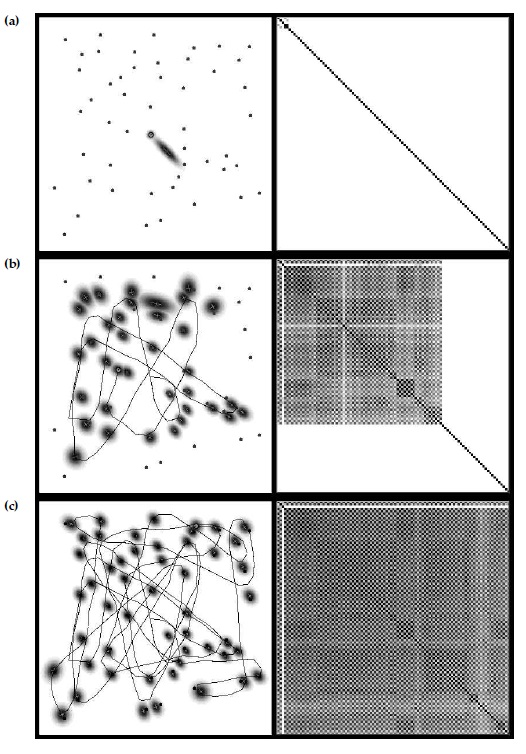
\includegraphics[width=0.9\linewidth]{104orig}}
	\caption{ ( Рис. 10.4 EKF SLAM с известной ассоциацией данных в имитационной среде. Карта показана слева, тон серого соответствует неопределённости каждого ориентира. Матрица справа – это матрица корреляции, нормализованная ковариационная матрица апостериорной оценки. После некоторого времени $x$- и все оценки $y$-координат становятся полностью коррелированны.)}
	\label{fig:104orig}
\end{figure}

\begin{figure}[H]
	\center{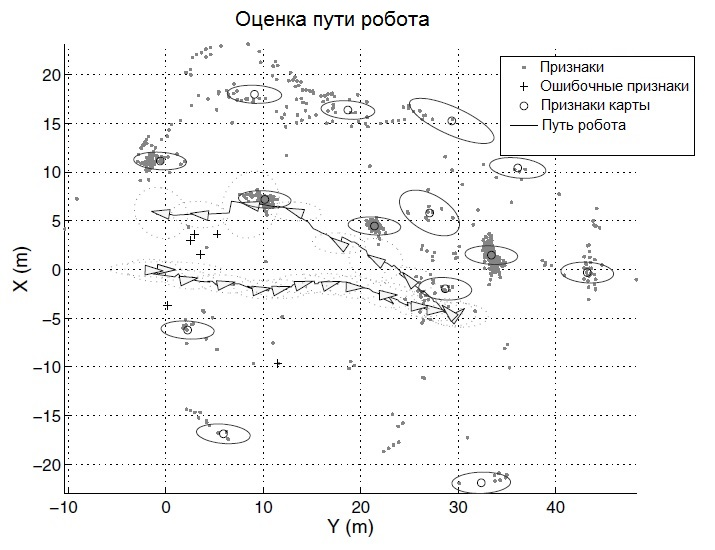
\includegraphics[width=0.9\linewidth]{105orig}}
	\caption{ ( Рис. 10.5 Пример оценки карты и положения робота фильтром Калмана. Изображение принадлежит Стефану Виллиамсу и Хью Дюрран-Уайту, Австралийский центр полевой робототехники (Stefan Williams and Hugh Durrant-Whyte, Australian Centre for Field Robotics).)}
	\label{fig:105orig}
\end{figure}

\begin{figure}[H]
	\center{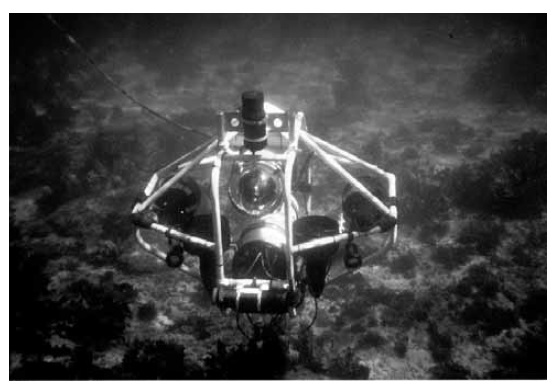
\includegraphics[width=0.9\linewidth]{106orig}}
	\caption{ ( Рис. 10.6 Подводный аппарат «Оберон», разработанный в университете Сиднея. Изображение принадлежит Стефану Виллиамсу и Хью Дюрран-Уайту, Австралийский центр полевой робототехники (Stefan Williams and Hugh Durrant-Whyte, Australian Centre for Field Robotics))}
	\label{fig:106orig}
\end{figure}

\begin{figure}[H]
	\center{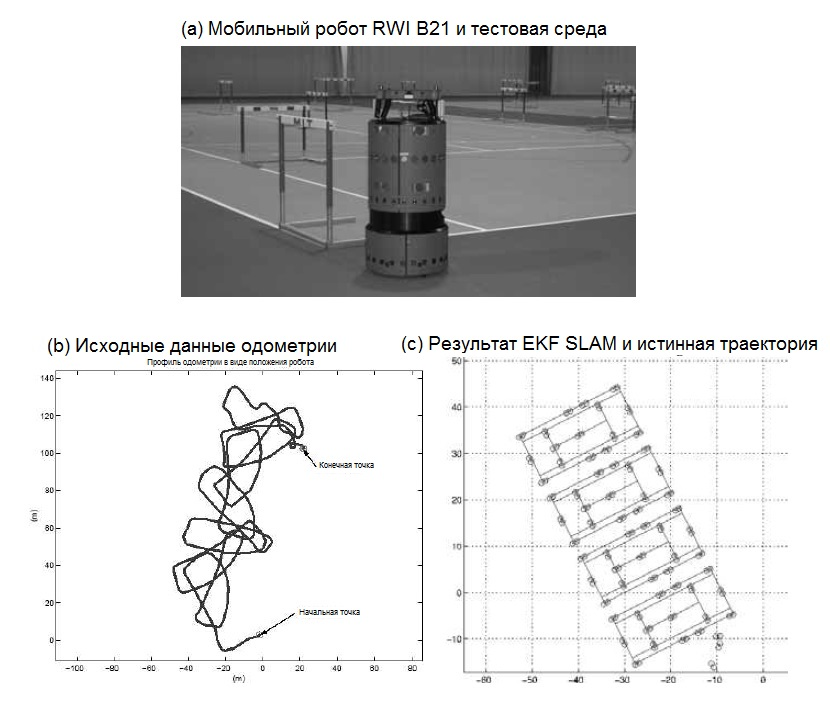
\includegraphics[width=1\linewidth]{107orig}}
	\caption{ ( Рис. 10.7 Мобильный робот MIT B21 на размеченной тестовой площадке(a). Исходная одометрия робота после прохода площадки в ручном режиме(b). Результатом работы EKF SLAM стала очень точная карта (c). Показана сгенерированная карта, наложенная поверх сконструированной вручную. Все изображения и результаты принадлежат Джону Леонарду и Мэтью Уолтеру, МИТ (John Leonard and Matthew Walter, MIT).)}
	\label{fig:107orig}
\end{figure}

На Рис. 10.7 показан результат другой реализации EKF SLAM. На врезке
(a)	показан мобильный робот RWI B21, разработанный в MIT в тестовой среде. Тестовой средой служит теннисный корт, переносные барьеры означают препятствиям, их положение было вручную определено с точностью порядка сантиметров для сравнения. На врезке (b) Рис. 10.7 показан пройденный путь по исходным данным одометрии. Результат работы EKF SLAM показан на врезке (c), наложенный на карту, сконструированную вручную. Читатель может убедиться, что сгенерированная карта очень точна.\\

\textbf{10.3.3	Выбор признаков и управление картой}\\

Обеспечение надёжности EKF SLAM на практике часто требует дополнительных методов управления картой. Во многих из них принимается во снимание нереалистичность допущения о гауссовом характере шума, а многие сомнительные измерения относят к более широким распределениям шумов. Такие сомнительные измерения могут привести к созданию ошибочных ориентиров на карте, которые, в свою очередь, отрицательно повлияют на локализацию робота.\\

ВЫБРОСЫ\\

Многие современные методы имеют механизмы обработки \textit{выбросов} в пространстве измерений. Такие выбросы определяются как сомнительные наблюдения ориентиров вне пределов диапазона неопределённости любых ориентиров на карте.\\

СПИСОК ВРЕМЕННЫХ ОРИЕНТИРОВ\\ 

Самым простым способом удалить такие выбросы является поддержка \textit{списка временных ориентиров}. Вместо дополнения карты новым ориентиром сразу поле того, как измерение покажет его обнаружение, такой ориентир сначала добавляется в список временных ориентиров. Этот список выглядит в точности как как карта, но не используется для уточнения положения робота (соответствующие градиенты в уравнениях измерения установлены нулевыми). Если ориентир наблюдается постоянно и размер эллипса неопределённости сильно уменьшается, ориентир переносится на рабочую карту. 

В практических реализациях этот механизм способен существенно уменьшить количество ориентиров на карте, при этом сохраняя все физические ориентиры, имеющие высокую вероятность.\\
ВЕРОЯТНОСТЬ СУЩЕСТВОВАНИЯ ОРИЕНТИРА\\
Дальнейшим шагом, также обычно используемым в современных методах, является поддержка \textit{вероятности существования ориентира.} Такая апостериорная вероятность может быть реализована в виде логарифма шансов и обозначаться $o_j$ для $j$-го ориентира на карте. Когда наблюдается $j$-ый ориентир $m_j$, $o_j$ увеличивается на фиксированное значение. Отсутствие наблюдения ориентира $m_j$, когда он должен быть в радиусе действия датчиков робота уменьшает $o_j$. Поскольку никогда нет полной уверенности, находится ли ориентир в радиусе действия датчиков робота, уменьшение можно выполнить в виде коэффициента вероятности. Ориентиры удаляются с карты, когда значение $o_j$ падает ниже установленного порога. Такие методы обычно позволяют создать карты значительно меньшего размера, учтя негауссовые шумы измерения.

Инициализация оценки для нового ориентира начинается с ковариации с большими элементами, как предлагается в выражении (10.9)\\
ЧИСЛОВАЯ НЕСТАБИЛЬНОСТЬ EKF SLAM\\

и может вызвать неустойчивость численного решения. Это происходит потому, что самый первый шаг обновления ковариации поменяет значение на несколько порядков, возможно слишком много для создания положительно определённой матрицы. Лучшей стратегией будет явное указание шага инициализации любого признака, который ранее не наблюдался. В частности, такой шаг может напрямую инициализировать ковариацию $\varSigma_t$  текущей неопределённостью ориентира вместо выполнения строки 24 в Таблице 10.2 (то же, что и среднее значение в строке 23).

Как отмечалось ранее, метод максимального правдоподобия для ассоциации данных имеет одно явное ограничение. Дело в том, что он отходит от идеи полной апостериорной оценки в вероятностной робототехнике. Вместо поддержки общего апостериорного распределения по дополненным векторам и ассоциации данных, максимум правдоподобия сводит проблему ассоциации данных к детерминированному определению, как если бы ассоциация по методу максимального правдоподобия была всегда верна. Это ограничение делает EKF чувствительным к ошибочной идентификации ориентиров и может привести к неверным результатам. На практике исследователи часто решают эту проблему выбором одного из двух описанных ниже методов, уменьшающих шансы перепутать ориентиры:\\

\textbf{•	Распределение в пространстве.} Чем дальше друг от друга расположены ориентиры, тем меньше шанс их спутать. Поэтому общепринятым методом является выбор ориентиров достаточно далеко друг от друга, чтобы вероятность их перепутать была мала. Это приводит к интересному компромиссу: большое количество ориентиров увеличивает шанс их перепутать, но слишком малое количество их число затрудняет локализацию робота. Об оптимальной плотности ориентиров пока известно мало, и исследователи часто полагаются на интуицию при выборе отдельных значений.\\

\textbf{•	Сигнатуры.} При выборе соответствующих ориентиров важно максимизировать их различимость при восприятии. Например, двери бывают разного цвета, а коридоры – имеют различную ширину. Результирующие сигнатуры важны для работы SLAM.\\

С такими дополнениями алгоритм EKF SLAM успешно применялся к большому количеству разных практических проблем картографирования, включая воздушные дроны, наземные и подводные.

Ключевое ограничение EKF SLAM лежит в необходимости выбора соответствующих ориентиров. При ограничении интерпретации данных с датчиков лишь наличием и отсутствием ориентиров, большое количество информации просто отбрасывается. Это приводит к потере данных в алгоритме SLAM, способный использовать датчики без предварительной фильтрации. Квадратичная зависимость времени обновления EKF ограничивает алгоритм относительно разреженными картами с менее чем 1000 признаков. На практике же часто необходимо стремиться к картам с $10^6$ признаков или более, в этом случае EKF неприменим.

Относительно малая размерность карты может усложнять проблему ассоциации данных. Это легко проверить: если открыть глаза и окинуть взглядом всю комнату, скорее всего, проблемы с ориентированием не возникнет! Однако, если иметь информацию только о небольшом количестве ориентиров,  например, о местоположении всех источников света, решение будет значительно затруднено. Поэтому, ассоциация данных в EKF SLAM более сложна по сравнению с некоторыми другими алгоритмами SLAM, обсуждаемыми в последующих главах, и способных обрабатывать на порядки больше признаков.\\ 
ОСНОВНАЯ ДИЛЕММА EKF SLAM\\
Это нашло отражение в \textit{основной дилемме EKF SLAM}: хотя инкрементная ассоциация данных по методу максимального правдоподобия может хорошо работать с плотными картами с сотнями миллионов признаков, она неустойчива на разреженных картах. Напротив, для EKF требуются разреженные карты в силу квадратичной сложности обновления. В последующих главах будут обсуждаться более эффективные алгоритмы SLAM, способные обрабатывать большие карты. Также будут обсуждаться более надёжные методы ассоциации данных. В силу большого количества ограничений  алгоритм EKF SLAM, представленный в этой главе, имеет, по большей части, исторический интерес.\\

\textbf{10.3	Вывод}\\

В данной главе описана общая задача SLAM и представлен метод EKF.\\

•	Задача SLAM определена как одновременная локализация и построение карты. Робот предпринимает попытки построить карту окружающей среды, с одновременным поиском своего местоположения на этой карте.\\

•	Задача SLAM имеет две версии: онлайновую и глобальную, при этом обе включают оценку карты. В онлайн задаче выполняется поиск текущего местоположения, а в глобальной – определение по всем положениям. Обе задачи одинаково важны на практике и хорошо освещены в литературе.\\

•	Алгоритм EKF SLAM, возможно самый лёгкий в реализации из всех известных, был успешно использован в онлайн задаче SLAM. Для известного соответствия в нем используется инкрементный подход и обновление требует времени, квадратично зависящего от числа ориентиров на карте.\\

•	Когда соответствия неизвестны, в алгоритме EKF SLAM используется инкрементальная функция оценки максимального правдоподобия. Результирующий алгоритм хорошо работает для ясно различимых между собой ориентиров.\\

•	Были описаны дополнительные методы управления картами. Две общепринятые стратегии идентификации выбросов включают  временный список  ориентиров, которые не наблюдаются достаточно часто, и счётчик количества наблюдений ориентира, вычисляющий апостериорную оценку существования ориентира.\\

•	EKF SLAM весьма успешно применялся для разнообразных проблем картографии в робототехнике. Основными недостатками являются необходимость приемлемого уровня различения ориентиров и вычислительная сложность обновления фильтра.\\

На практике EKF SLAM использовался с некоторым успехом. Когда ориентиры достаточно различимы, апостериорная оценка вычисляется достаточно хорошо. Преимуществом полной апостериорной оценки является именно её полнота, поскольку учитывается полная неопределённость, что позволяет роботу оценивать воздействие управления, и принимать во внимание истинную неопределённость. Однако, алгоритм EKF SLAM страдает от чрезмерно высокой вычислительной сложности и ограничения применения только разреженных карт. Это, в свою очередь, затрудняет проблему ассоциации данных, и EKF SLAM имеет склонность к сбоям в ситуациях, когда ориентиры неразличимы. Ещё большая неустойчивость вызвана тем, что алгоритм EKF SLAM основан на методе инкрементной ассоциации данных методом максимального правдоподобия. Этот метод делает невозможным пересмотр прошлой ассоциации данных, и может вызвать сбой при неверной ассоциации данных.

Алгоритм EKF SLAM применяется не только для онлайн задачи SLAM, но и для полной задачи SLAM. В полной задаче SLAM добавление нового положения к вектору состояний на каждом такте времени вызывает бесконтрольный рост как вектора состояний, так и ковариации. Обновление ковариации требует все больше времени и метод быстро выходит из приемлемого диапазона, вне зависимости от скорости процессора.\\

\textbf{10.4	Библиографические примечания}\\

Проблема SLAM появилась за много столетий до современной робототехники. Проблема моделирования физической структуры среды с движущейся платформы датчика лежит в основе целого ряда направлений, таких, как науки о Земле, фотограмметрия и компьютерное зрение. Многие из математических методов, лежащие в основе  сегодняшнего SLAM, изначально были разработаны для вычисления планетных орбит. Например, метод наименьших квадратов можно проследить до работ Иоганна Карла Фридриха Гаусса (Johann Carl Friedrich Gauss, 1809). SLAM – это, в основном, задача географического исследования. Применительно к роботу, это приводит к возникновению проблем, с которыми исследователи-люди сталкиваются редко, например, как проблема назначения соответствия и соответствующих признаков.

В робототехнике проблема EKF в SLAM была впервые представлена в серии основополагающих работ Чизмана и Смита (Cheeseman and Smith, 1986), Смита и Чизмана (Smith and Cheeseman, 1986), Смита (Smith et al., 1990). В этих работах впервые был описан метод EKF, обсуждаемый в данной главе. Также, как и в этой книге, Смит обсуждал EKF в контексте картографирования на основе признаков с точечными ориентирами и известной ассоциацией данных. Первые реализации EKF SLAM были выполнены Маутарлиром и Чатила (Moutarlier and Chatila, 1989a, b) и Леонардом и Дюран-Уайтом (Leonard and Durrant-Whyte, 1991) и в некоторых из них в качестве ориентиров использовались искусственные метки. EKF стал модным, когда многими авторами были исследованы альтернативные методы поддержания точной оценки положения при картографировании (Cox, 1991). Ранняя работа Дикманса и Грэфи (Dickmanns and Graefe, 1988) по оценке кривизны дороги в автономных автомашинах имеет самое прямое отношение к проблеме, детальную информацию для ознакомления можно найти в работе (Dickmanns, 2002).

Как показывают последние работы, SLAM очень активно исследуется (Leonard et al. 2002b). Большой объем литература по SLAM (или CML, что значит "concurrent mapping and localization" – конкурентное картографирование и локализация, как его назвали Леонард и Дюран-Уайт (Leonard and Durrant-Whyte,1991)), можно найти в работах Труна (Thrun, 2002). Важность поддержания корреляций на карте была отмечена Цорба (Csorba, 1997), который в своей кандидатской диссертации также установил некоторые основные результаты конвергенции. После этого усилиями многих авторов основная парадигма была дополнена самыми различными методами. Методы управления признаками, описанные в данной главе, были впервые описаны Диссанаяки (Dissanayake et al., 2001, 2002), а также Бейли (Bailey, 2002). Вильямс (Williams et al., 2001) разработал идею временных списков признаков в SLAM для уменьшения эффекта ошибок обнаружения признаков. Инициализация признаков обсуждалась в работе Леонарда (Leonard et al., 2002a), который в явном виде сохранял оценку предыдущих положений для использования датчиков, которые предоставляли неполные данные координат признаков. Представление, предотвращающее появление пересечений явной факторизацией «отклонений» от апостериорного распределения, было выведено Кастелланосом (Castellanos et al., 1999), и показало улучшение вычислительной стабильности базового EKF. Янсфельт (Jensfelt et al., 2002) открыл способ существенного улучшения для SLAM внутри помещений при использовании базовых геометрических ограничений, таких, как параллельность и перпендикулярность большинства стен.  Ранние работы по SLAM с использованием сонаров восходят к Ренкену (Rencken (1993). Современная система SLAM с ультразвуковыми датчиками была описана Тардос (Tardós et al., 2002). Кастелланос (Castellanos et al., 2004) выполнил критический анализ целостности EKF. Эмпирическое сравнение нескольких алгоритмов можно найти в работах Ваганай (Vaganay et al., 2004). Некоторые открытые вопросы обсуждались Салихом и Морено (Salichs and Moreno, 2000). Исследование важной проблемы ассоциации данных будет описано в следующей главе (см. стр. 481 ???).

Как было отмечено, ключевым ограничением решения EKF в проблеме SLAM является квадратичность матрицы ковариации, что не осталось незамеченным. В последние годы множество исследователей предлагали алгоритмы EKF SLAM, которые стали заметно лучше масштабируемыми с помощью разбиения карты на вложенные карты с раздельным сохранением ковариаций. Некоторые из оригинальных работ в этой области принадлежат Леонарду и Федеру (Leonard and Feder, 1999), Гюванту и Неботу (Guivant and Nebot, 2001), а также Вильямсу (Williams, 2001). Леонард и Федер (Leonard and Feder, 1999) ввели алгоритм несвязанного стохастического картографирования с разбиением карты на несколько отдельных, более управляемых карт меньшего размера. Этот подход вычислительно эффективен, но не обеспечивает механизма распространения информации через сеть локальных карт (Leonard and Feder 2001). Гювант и Небот (Guivant and Nebot, 2001, 2002), наоборот, выполнили приблизительную факторизацию матрицы ковариации, что позволило существенно уменьшить сложность обновления EKF. Вильямс (Williams (2001, Williams et al., 2002) предложил ограниченный локальный фильтр вспомогательных карт (constrained local submap filter - CLSF), основанный на создании независимых локальных вспомогательных карт признаков в непосредственной близости от транспортного средства. Вильямс (Williams et al., 2002) привёл результаты картографирования для подводной среды (на Рис. 10.5 приводится одна из его ранних работ). Методы последовательного объединения карт (sequential  map joining techniques) описанные Тардосом (Tardós et al., 2002) являются относительной декомпозицией. Бейли (Bailey, 2002) вывел похожий метод, представив карты SLAM в иерархическом виде. Фолкессон и Кристенсен (Folkesson and Christensen, 2003) описали метод, в котором частые обновления затрагивали только область вблизи робота, а оставшаяся часть карты обновлялась значительно реже. Все эти методы достигли той же скорости сходимости, как полное решение EKF, за исключением затруднений в виде вычисления операций сложности O(n2). Тем не менее, они значительно лучше масштабируемы для больших задач с десятками тысяч признаков.

Некоторые исследователи разработали гибридные методы SLAM, комбинирующие EKF SLAM с пространственными подходами, например, картами сеток занятости. Гибридная метрическая карта (hybrid metric map -HYMM), предложенная Гювантом (Guivant et al., 2004) и Нието (Nieto et al., 2004) разбивает карты на треугольные области (LTR) используя в качестве основного отображения этих областей пространственные карты, такие, как карты сеток занятости. Эти локальные карты комбинируются с помощью EKF. Бургард (Burgard et al., 1999b) также выполнял разбиение карт на локальные карты сеток занятости, но использовал алгоритм максимизации ожидания (expectation maximization- EM) (см Dempster et al., 1977) для комбинированя локальных карт в общую глобальную. В работе Бетги-Брезетца (Betgé-Brezetz et al., 1995, 1996) в парадигму SLAM были интегрированы сразу два типа отображений: растровые карты для представления сред вне помещений, и объектное представление для разреженных объектов вне помещений.

Обобщение SLAM для динамических сред можно найти в работах Ванга (Wang et al., 2003), Хунела (Hähnel  et al., 2003c), а также Вольфа и Сухатми (Wolf and Sukhatme, 2004). Ванг (Wang et al., 2003) разработал алгоритм под названием "SLAM с DATMO", сокращение для «SLAM with the detection and tracking of moving objects» (SLAM с обнаружением и отслеживанием движущихся объектов). Их подход основывался на EKF, но позволял перемещение признаков. Хёнел (Hähnel et al., 2003c) изучил задачу применения SLAM в средах с множеством движущихся объектов. Они успешно применили алгоритм EM для фильтрации измерений, которые, вероятнее всего, относились к движущимся объектам. Таким образом, им удалось получить карты для сред, непригодных для обычных методов SLAM. В методе Вольфа и Сухатми (Wolf and Sukhatme, 2004) сохранялись две связанные сетки занятости окружающей среды, одна для статической карты, а вторая – для движущихся объектов. Локализация выполнялась алгоритмов наподобие SLAM с регулярными ориентирами.

SLAM системы позволили создать множество практических реализаций. Рикоски (Rikoski et al.,2004) применил SLAM к одометрии подводной лодки с помощью сонара, представив новый метод «звуковой одометрии». Использование SLAM в для составления карт заброшенных шахт было описано Нуктером (Nüchter et al., 2004), который обобщил парадигму до полной оценки положения по шести измерениям. Обобщения проблемы SLAM для нескольких роботов также были предложены рядом исследователей. Некоторые из ранних работ принадлежат Неттлетону (Nettleton et al., 2000), разработавшему метод, в котором роботы сохраняли локальные карты EKF, но соединяли их на основе информационного выражения апостериорного распределения. Альтернативный метод принадлежит Реклеитису (Rekleitis et al., 2001a), который использовал группы неподвижных и движущихся роботов для уменьшения ошибки локализации при выполнении SLAM. Фенвик (Fenwick et al., 2002) представил полное теоретическое исследование слияния карт нескольких роботов, в частности SLAM на основе ориентиров. Методы слияния проходов сканирования были разработаны Конолигом (Konolige et al., 1999) и Труном (Thrun et al. (2000b, 2001).\\

СТРУКТУРА ИЗ ДВИЖЕНИЯ\\

Ряд исследователей предложили SLAM системы для определённых наборов датчиков. Важным видом датчика является видеокамера, но она способна измерять только угол направления на признаки. Эта задача хорошо изучена в литературе по компьютерному зрению под названием "структура из движения" (structure from motion- SFM) (Tomasi and
Kanade 1992; Soatto and Brockett 1998; Dellaert et al. 2003), и в области фотограмметрии (Konecny, 2002). В SLAM фундаментальная работа по SLAM, с использованием только лишь угла направления принадлежит Динсу и Герберту (Deans and Hebert, 2000, 2002). В их методе выполняется рекурсивная оценка признаков среды, инвариантных для положения робота, для отделения ошибки положения от ошибок карты. Большое количество исследователей применяли SLAM с камерами в качестве основного датчика (Neira et al. 1997; Cid et al. 2002; Davison 2003). Дэвисон (Davison, 1998) предложил метод активного зрения в контексте SLAM. Работа Дудека и Егерссура (Dudek and Jegessur, 2000) основана на распознавании места по внешнему виду, а Хайет (Hayet et al., 2002) и Бугет и Перона (Bouguet and Perona, 1995) использовали для этого визуальные ориентиры. Дибел (Diebel et al., 2004) разработал фильтр для SLAM с активным стерео датчиком, который учитывал нелинейное распределение шумов стерео датчика расстояния. Методы слияния показаний датчиков в SLAM были разработаны Деви и Булата (Devy and Bulata, 1996). Кастелланос (Castellanos et al., 2001) эмпирически обнаружил, что слияние сигналов лазера и камеры даёт лучшие результаты по сравнению с их раздельным использованием.

SLAM также было обобщено для проблемы построения плотных трёхмерных моделей. Ранние системы получения трёхмерных моделей для мобильных роботов, действующих внутри помещений, можно найти в работах Рида и Аллена (Reed and Allen, 1997), Иоччи (Iocchi et al., 2000), Труна (Thrun et al., 2004b). Деви и Парра (Devy and Parra, 1998) получали трёхмерные модели на основе параметрических кривых. Жао и Шибасаки (Zhao and Shibasaki, 2001), Теллер (Teller et al., 2001) и Фрах и Захор (Frueh and Zakhor, 2003) разработали весьма эффективные системы для построения больших текстурированных  трёхмерных карт городской среды. Ни одна из этих систем не применялась для проблемы SLAM вне помещений, поскольку имелись системы на основе GPS, но они плотно связаны с математической основой SLAM. Эти методы хорошо сочетаются с множеством работ по реконструкции городских сред по аэрофотоснимкам (Jung and Lacroix 2003; Thrun et al. 2003).

В последующих главах описаны альтернативы простым методам EKF. В описанных подходах используются многие уже упоминавшиеся соображения относительно обобщений, поэтому становится почти невозможно провести границы между разными типами фильтров. Литературный обзор будет продолжен в конце следующей главы, при обсуждении алгоритма SLAM, на основе выражения из теории информации.\\

\textbf{10.5	Упражнения}\\

1.	Какова вычислительная сложность обновления движения в EKF SLAM? Использовать нотацию $O(\,\,)$. Сравнить с наихудшей сложностью EKF с вектором признаков аналогичного размера.\\

SLAM ТОЛЬКО ПО НАПРАВЛЕНИЮ\\
2.	 SLAM только по направлению относится к задаче SLAM, когда датчики способны определить только направление на ориентир, но не расстояние до него. Как было отмечено, SLAM только по направлению тесно связан со подходом "структуры из движения" (SFM) в компьютерном зрении. Одна из задач SLAM только по направлению на основе EKF касается инициализации оценки местоположения ориентира, даже если соответствия известны. Обсудить, почему это происходит и вывести метод инициализации оценки местоположения ориентира (в виде математического ожидания и ковариации), применимый для SLAM только по направлению.\\

3.	На странице 329 ??? было отмечено, что алгоритм EKF из Таблицы 10.2 может стать вычислительно нестабильным. Вывести метод явной установки значений $\mu_t$ и $\varSigma_t$ когда новый признак наблюдается впервые. Такой метод может не потребовать инициализации очень большим значением ковариации. Показать, что результат математически эквивалентен строкам 23 и 24, где ковариация инициализирована выражением (10.9).\\

4.	В тексте предлагается использовать бинарный байесовский фильтр для вычисления вероятности того, что ориентир, выраженный в апостериорном распределении, действительно существует в физическом мире.\\

(a)	В первой части упражнения требуется разработать такой бинарный байесовский фильтр.\\

(b)	Теперь необходимо обобщить фильтр для ситуации, когда ориентиры спорадически исчезают с вероятностью $p^*$.\\

(c)	Представим ситуацию, когда для точно определённого ориентира долгое время не поступало информации о его существовании (ни положительной, ни отрицательной). До какого значения сойдётся фильтр? Доказать ответ.\\

5.	Представленный в данной главе алгоритм EKF SLAM неспособен решить проблему ассоциации данных в статистически непротиворечивой манере. Предложить алгоритм (и  аппарат статистики) для апостериорной оценки с неизвестной ассоциацией данных, представляющей апостериорное распределение в виде смеси гауссовых функций. Охарактеризовать его преимущества и недостатки. Как сложность апостериорного распределения возрастает со временем?\\

6.	Основываясь на предыдущей проблеме, разработать приближенный метод апостериорной оценки с неизвестной ассоциацией данных, в котором время, необходимое для каждого инкрементного шага обновления, не увеличивается со временем (считая количество ориентиров постоянным).\\

7.	Разработать алгоритм фильтра Калмана, использующего в качестве основных компонентов локальные карты сеток занятости, а не ориентиры.  Среди прочего, необходимо решить, как локальные сетки связаны друг с другом и что делать с все возрастающим числом локальных сеток.\\  








 
\end{document}